\def\paperversiondraft{draft}
\def\paperversionnormal{normal}

% If the paper version is set to 'normal' mode keep it,
% otherwise set it to 'draft' mode.
\ifx\paperversion\paperversionnormal
\else
  \def\paperversion{draft}
\fi

\documentclass[conference]{IEEEtran}
\IEEEoverridecommandlockouts

\def\acmversionanonymous{anonymous}
\def\acmversionjournal{journal}
\def\acmversionnone{none}

\def\acmversion{anonymous}

\usepackage{colortbl}

% 'draftonly' environment
\usepackage{environ}
\ifx\paperversion\paperversiondraft
\newenvironment{draftonly}{}{}
\else
\NewEnviron{draftonly}{}
\fi

% Most PL conferences are edited by conference-publishing.com. Follow their
% advice to add the following packages.
%
% The first enables the use of UTF-8 as character encoding, which is the
% standard nowadays. The second ensures the use of font encodings that support
% accented characters etc. (Why should I use this?). The mictotype package
% enables certain features 'to­wards ty­po­graph­i­cal per­fec­tion
\usepackage[utf8]{inputenc}
\usepackage[T1]{fontenc}
\usepackage{microtype}
\usepackage{tcolorbox}

\ifx\paperversion\paperversiondraft
  \usepackage{geometry}
\fi
\usepackage{xargs}
\usepackage{lipsum}
\usepackage{xparse}
\usepackage{xifthen, xstring}
\usepackage{xspace}
\usepackage{marginnote}
\usepackage{etoolbox}
\usepackage[acronym,shortcuts]{glossaries}
\usepackage{amsmath}
\usepackage{amssymb}
\usepackage{hyperref}
\usepackage{amsthm}   % \theoremstyle/\newtheorem; acmart loaded this
\usepackage{thmtools} % required for autoref to lemmas
\usepackage{algorithm}
\usepackage[noend]{algpseudocode}
\usepackage{hyphenat}
\usepackage[shortcuts]{extdash}

\input{tex/setup.tex}

\usepackage[numbers]{natbib}
\bibliographystyle{IEEEtranN}

\usemintedstyle{colorful}

% Newer versions of minted require the 'customlexer' argument for custom lexers
% whereas older versions require the '-x' to be passed via the command line.
% \makeatletter
% \ifcsdef{MintedExecutable}
% {
%   % minted v3
%   \newminted[mlir]{tools/lexers/MLIRLexer.py:MLIRLexerOnlyOps}{mathescape}
%   \newminted[xdsl]{tools/lexers/MLIRLexer.py:MLIRLexer}{mathescape, style=murphy}
%   \newminted[lean4]{tools/lexers/Lean4Lexer.py:Lean4Lexer}{mathescape, breaklines}
% }
% {
%   \ifcsdef{minted@optlistcl@quote}
%   {
%     \newminted[mlir]{tools/lexers/MLIRLexer.py:MLIRLexerOnlyOps}{customlexer, mathescape}
%     \newminted[xdsl]{tools/lexers/MLIRLexer.py:MLIRLexer}{customlexer, mathescape, style=murphy}
%     \newminted[lean4]{tools/lexers/Lean4Lexer.py:Lean4Lexer}{customlexer, mathescape, breaklines}
%   }
%   {
%     \newminted[mlir]{tools/lexers/MLIRLexer.py:MLIRLexerOnlyOps -x}{mathescape}
%     \newminted[xdsl]{tools/lexers/MLIRLexer.py:MLIRLexer -x}{mathescape, style=murphy}
%     \newminted[lean4]{tools/lexers/Lean4Lexer.py:Lean4Lexer -x}{mathescape, breaklines}
%   }
% }
% \makeatother

% We use the following color scheme
%
% This scheme is both print-friendly and colorblind safe for
% up to four colors (including the red tones makes it not
% colorblind safe any more)
%
% https://colorbrewer2.org/#type=qualitative&scheme=Paired&n=4

\definecolor{pairedNegOneLightGray}{HTML}{cacaca}
\definecolor{pairedNegTwoDarkGray}{HTML}{827b7b}
\definecolor{pairedOneLightBlue}{HTML}{a6cee3}
\definecolor{pairedTwoDarkBlue}{HTML}{1f78b4}
\definecolor{pairedThreeLightGreen}{HTML}{b2df8a}
\definecolor{pairedFourDarkGreen}{HTML}{33a02c}
\definecolor{pairedFiveLightRed}{HTML}{fb9a99}
\definecolor{pairedSixDarkRed}{HTML}{e31a1c}

\createtodoauthor{grosser}{pairedOneLightBlue}
\createtodoauthor{sam}{pairedTwoDarkBlue}
\createtodoauthor{osman}{pairedThreeLightGreen}
\createtodoauthor{sid}{pairedFourDarkGreen}
\createtodoauthor{authorFive}{pairedFiveLightRed}
\createtodoauthor{authorSix}{pairedSixDarkRed}

\newacronym{ir}{IR}{Intermediate Representation}
\newacronym{fa}{FA}{full-adder}
\newacronym{ha}{HA}{half-adder}
\newacronym{cpa}{CPA}{carry-propagate adder}
\newacronym{lsb}{LSB}{least-significant bit}
\newacronym{msb}{MSB}{most-significant bit}
\newacronym{sca}{SCA}{Symbolic Computer Algebra}
\newacronym{hls}{HLS}{High-level Synthesis}
\newacronym{asic}{ASIC}{application-specific integrated circuits}
\newacronym{cse}{CSE}{Common Subexpression Elimination}
\newacronym{aig}{AIG}{AND-Inverter Graph}
\newacronym{sop}{SOP}{Sum-of-Products}

\newcommand{\sem}[1]{\llbracket #1 \rrbracket}
% Denotation of a BitExpr under the bit environment sigma. The heap denotation
% keeps its \mathcal{H} prefix to distinguish it from the bare BitExpr brackets.
\newcommand{\csem}[1]{\sem{#1}_{\sigma}}
\newcommand{\val}[1]{\mathrm{val}(#1)} 
% \newcommand{\bvsem}[1]{\mathcal{B}\llbracket #1 \rrbracket_{\rho}}
\newcommand{\bvsem}[1]{\llbracket #1 \rrbracket_{\rho}}
% \newcommand{\hsem}[1]{\mathcal{\textsc{}H}\llbracket #1 \rrbracket_{\sigma}}
\newcommand{\hsem}[1]{\llbracket #1 \rrbracket_{\sigma}}
\newcommand{\BitExpr}{\ensuremath{\texttt{BitExpr}}\xspace}
\newcommand{\Col}{\ensuremath{\texttt{Column}}\xspace}
\newcommand{\Heap}{\ensuremath{\texttt{BitHeap}}\xspace}
\newcommand{\Arith}{\ensuremath{\texttt{ArithCircuit}}\xspace}
\newcommand{\Step}{\ensuremath{\texttt{Step}}\xspace}
\newcommand{\Chain}{\ensuremath{\texttt{Chain}}\xspace}
\newcommand{\Vect}{\ensuremath{\texttt{Vector}}\xspace}
\newcommand{\var}{\mathsf{var}}
\newcommand{\HA}{\mathsf{HA}}
\newcommand{\FA}{\mathsf{FA}}
\newcommand{\maj}{\mathsf{maj}}
\newcommand{\zext}{\mathsf{zext}}
\newcommand{\trunc}{\mathsf{trunc}}
\newcommand{\flatten}[1]{\lfloor #1 \rfloor}
\newcommand{\lift}[1]{\lceil #1 \rceil}
\newcommand{\compile}[1]{\langle\!\langle #1 \rangle\!\rangle}

\newcommand{\geoAreaThirtyTwo}{1.17}
\newcommand{\geoDelayThirtyTwo}{1.14}
\newcommand{\geoAreaSixteen}{1.19}
\newcommand{\geoDelaySixteen}{1.12}
\newcommand{\geoAreaEight}{1.19}
\newcommand{\geoDelayEight}{1.10}

\graphicspath{{./images/}}
\usepackage{subcaption}

% Define macros that are used in this paper
%
% We require all macros to end with a delimiter (by default {}) to enusure
% that LaTeX adds whitespace correctly.
\makeatletter
\newcommand\requiredelimiter[2][########]{%
  \ifdefined#2%
    \def\@temp{\def#2#1}%
    \expandafter\@temp\expandafter{#2}%
  \else
    \@latex@error{\noexpand#2undefined}\@ehc
  \fi
}
\@onlypreamble\requiredelimiter
\makeatother

\newcommand\newdelimitedcommand[2]{
\expandafter\newcommand\csname #1\endcsname{#2}
\expandafter\requiredelimiter
\csname #1 \endcsname
}

\newdelimitedcommand{toolname}{Tool}

\usepackage{booktabs}
\newcommand{\ra}[1]{\renewcommand{\arraystretch}{#1}}

\usepackage[verbose]{newunicodechar}
\newunicodechar{₁}{\ensuremath{_1}}
\newunicodechar{₂}{\ensuremath{_2}}
\newunicodechar{∀}{\ensuremath{\forall}}
\newunicodechar{α}{\ensuremath{\alpha}}
\newunicodechar{β}{\ensuremath{\beta}}

% \circled command to print a colored circle.
% \circled{1} pretty-prints "(1)"
% This is useful to refer to labels that are embedded within figures.
\DeclareRobustCommand{\circled}[2][]{%
    \ifthenelse{\isempty{#1}}%
        {\circledbase{pairedOneLightBlue}{#2}}%
        {\autoref{#1}: \hyperref[#1]{\circledbase{pairedOneLightBlue}{#2}}}%
}

% listings don't write "Listing" in autoref without this.
\providecommand*{\listingautorefname}{Listing}
\providecommand*{\sectionautorefname}{Section}
\providecommand*{\subsectionautorefname}{Section}
\providecommand*{\subsubsectionautorefname}{Section}
\renewcommand{\sectionautorefname}{Section}
\renewcommand{\subsectionautorefname}{Section}
\renewcommand{\subsubsectionautorefname}{Section}
\usepackage{stmaryrd}
\newcommand{\bit}[2]{\llbracket #1 \rrbracket_{#2}}

% acmart predefined these; IEEEtran does not.
\theoremstyle{plain}
\newtheorem{theorem}{Theorem}
\newtheorem{lemma}[theorem]{Lemma}
\newtheorem{corollary}[theorem]{Corollary}
\theoremstyle{definition}
\newtheorem{definition}[theorem]{Definition}
\providecommand*{\theoremautorefname}{Theorem}
\providecommand*{\definitionautorefname}{Definition}
\providecommand*{\lemmaautorefname}{Lemma}

% acmart provided these; IEEEtran does not.
\providecommand{\keywords}[1]{\par\noindent\textbf{Keywords:} #1}
\providecommand{\ccsdesc}[2][]{}
\providecommand{\settopmatter}[1]{}
\providecommand{\received}[2][]{}

\newcommand{\SynthesisSpeedupGeomean}{\ensuremath{X \times}}
\newcommand{\PerformanceSlowdownGeomean}{\ensuremath{Y \times}}


\begin{document}

%% Title information
\title{Correct-by-Construction Compressor Trees for Datapath Synthesis}

%% Author information
%% Contents and number of authors suppressed with 'anonymous'.
%% Each author should be introduced by \author, followed by
%% \authornote (optional), \orcid (optional), \affiliation, and
%% \email.
%% An author may have multiple affiliations and/or emails; repeat the
%% appropriate command.
%% Many elements are not rendered, but should be provided for metadata
%% extraction tools.
%% Author information (IEEEtran format).
%% Anonymized for review; restore the real block for camera-ready.
\ifx\acmversion\acmversionanonymous
\author{\IEEEauthorblockN{Anonymous Author(s)}}
\else
\author{%
  \IEEEauthorblockN{First1 Last1}
  \IEEEauthorblockA{%
    \textit{Department1} \\
    \textit{Institution1} \\
    City1, Country1 \\
    first1.last1@inst1.edu}
  \and
  \IEEEauthorblockN{First2 Last2}
  \IEEEauthorblockA{%
    \textit{Department2a} \\
    \textit{Institution2a} \\
    City2a, Country2a \\
    first2.last2@inst2a.com}
}
\fi

%% IEEEtran requires \maketitle before the abstract (acmart wanted it after).
\maketitle


\begin{abstract}
% An abstract should consist of six main sentences:
%  1. Introduction. In one sentence, what’s the topic?
Datapath circuits are the core computational units of digital designs and one of the most timing-critical parts of the design.
%  2. State the problem you tackle.
To meet the performance requirements, datapath circuits are aggressively optimized by synthesis tools.
These automatic datapath optimizations, like the deployment of compressor trees, make it hard to verify that the synthesized netlist implements the correct computation.
%  3. Summarize (in one sentence) why nobody else has adequately answered the research question yet.
Existing methods largely focus on verifying this post-synthesis netlist but either do not scale to large bit widths or
struggle to recover the circuit structure that optimizations destroyed.
%  4. Explain, in one sentence, how you tackled the research question.
We however, tackle the verification problem during synthesis. 
Rather than verifying the netlist post-synthesis, 
we construct it in an interactive theorem prover, 
synthesizing a provably correct-by-construction netlist.
% Our insight is that these methods attempt to tackle the verification problem at the wrong stage.
% They are all post-synthesis, where the structure of the circuit optimization has already been lost.
% Instead, we propose a pre-synthesis approach, where we build a formally verified
% synthesis pipeline built on interactive theorem proving.
% This eliminates the need for an expensive post-synthesis verification,
% instead leveraging the ability to implement correct-by-construction algorithms in a theorem prover.
%  5. In one sentence, how did you go about doing the research that follows from your big idea.
We formalize the bit heap data structure and two compressor tree construction algorithms in Lean 4,
letting us prove the correctness of key synthesis steps for any design we might encounter.
We integrate our formalized datapath synthesis engine with the CIRCT framework, which, 
when applied to datapath benchmarks, verifies 11 circuits that state-of-the-art verification tools cannot. 
% For this approach, we phrase circuit synthesis as a bit-heap compression problem.
% We formalize the bit heap data structure and its operations in the Lean theorem prover,
% synthesize compression trees with this data structure,
% and prove the correctness of these optimizations and datapath synthesis as a whole.
% Furthermore, our framework produces circuits that are consumed by the CIRCT framework, 
% that when applied to real world circuit designs, are \SynthesisSpeedupGeomean{} faster
% in synthesis plus verification time \sam[on]{grammar feels off} state-of-the-art verificiation tools,
% while only being \PerformanceSlowdownGeomean{} slower than the state of the art synthesis.
%  6. As a single sentence, what’s the key impact of your research?
% Overall, our approach lays down the foundations of verified datapath circuit synthesis.
% This demonstrates that our approach provides orders of magnitude speedup on verification,
% while not \sam[sacrificing performance]{Runtime performance yes - circuit quality which feels like a measure of perf for a synthesis tool - I would not claim.}. 
% Overall, our approach lays down the foundations for fast, performant datapath circuit synthesis.\sam{Surely the focus is correct/verified not fast and performant - what does performant mean here - before it meant runtime now it means circuit quality?}
% (http://www.easterbrook.ca/steve/2010/01/how-to-write-a-scientific-abstract-in-six-easy-steps/)

\end{abstract}

%% IEEE keywords. The ACM CCS concept block has no IEEE equivalent and was
%% dropped; IEEE venues use index terms instead.
\begin{IEEEkeywords}
Formal Verification, Datapath, Theorem Provers
\end{IEEEkeywords}

\section{Introduction}
Datapath circuits are a fundamental component of digital systems, responsible from performing computations on incoming data.
Thanks to advances in automatic datapath synthesis~\cite{Zimmermann2003OptimizedSum-of-products,Zimmermann2009DatapathDesign},
most datapath circuits can now be implemented using bitvector-level arithmetic.
Modern synthesis tools can map entire arithmetic expressions to highly optimized gate-level circuits, or netlists, that effectively
remove the computation of intermediate results. 
In this paper, we prove that this automatic datapath synthesis produces functionally correct netlists.     

One of the key datapath optimizations applies to bitvector addition with $N$ addends, an operation that is used to build nearly all multiplier circuits. 
In \ac{asic} design, recursively summing $N$ addends is slow because the delay of a binary \ac{cpa} depends on the bitwidth of the addends. 
Datapath synthesis improves this circuit's delay by reducing $N$ addends to two using a compressor tree comprised of many full- and half-adders~\cite{wallace_tree, application_specific_arithmetic}.
The compressor tree performs the reduction of the addends in parallel and is followed by a single \ac{cpa}, avoiding the need for sequential \acp{cpa} to compute the sum.
Compressor trees can be used to implement arbitrary sums of products, e.g., $a*b + 255*c - d$, and modern synthesis tools now automatically recognize and replace such sub-circuits during datapath synthesis. 
Whilst efficient and widely used, compression trees usually have highly irregular structures increasing the difficulty of verifying the generated circuits.\sam{CITE something}

Techniques exist to verify datapath circuits, including \ac{sca}~\cite{trace,mertcan_acl2multipliers,sca,kleinekathofer2026conflict,mahzoon2021revsca,kaufmann2019verifying}
and SAT-based methods~\cite{kaufmann2019verifying}.
One shortcoming of these methods is that the verification tool itself is almost always unverified, with the exception of~\cite{mertcan_acl2multipliers}.
A second shortcoming is that they do not scale to large and complex circuits, either due to state-space explosion in the SAT approach or polynomial explosion in \ac{sca}.
So checking that a synthesized datapath circuit is correct remains challenging, even today. 

We propose a different approach, verifying the synthesis step itself, rather than verifying the generated circuits.
This approach guarantees that the generated circuits are correct-by-construction, and scales to large circuits.
To prove this datapath synthesis step correct we formalize the bit heap data structure~\cite{arithmetic_core_generation_bitheaps,application_specific_arithmetic} and compression algorithms~\cite{dadda_tree} in the Lean~4 theorem prover~\cite{moura2021lean}.
To demonstrate that verified synthesis is competitive, we integrate the Lean-based datapath generator into an existing open-source synthesis tool.

Our contributions are:
\begin{itemize} 
  \item formalization of the bit heap data structure and efficient compression algorithms in a theorem prover (\autoref{sec:formalization}),
  \item integration into an existing synthesis flow to provide formally verified datapath circuits (\autoref{sec:integration}),
  \item the first verified synthesis of existing benchmarks using open-source tools (\autoref{sec:evaluation}). 
\end{itemize}

\section{Background}\label{sec:background}
In digital arithmetic, an unsigned integer bitvector, $x$, of length $n$ represents a sum of weighted bits $x = \sum_{i=0}^{n-1} 2^i \cdot x_i $,
where $x_i$ denotes the $i^{\textrm{th}}$ bit of $x$.
The multiplication of two length $n$ bitvectors can of course also be represented as a sum of weighted bits:
\[
    x \cdot y = \sum_{i=0}^{n-1} \sum_{j=0}^{n-1} 2^{i+j} \cdot x_i \cdot y_j
\]
where the term $x_i \cdot y_j$ is the logical AND of the bits, and the weight of the resulting bit is $2^{i+j}$. 
More complex partial product encodings exist~\cite{application_specific_arithmetic}, but they can all eventually be reduced to a sum of weighted bits. 

\begin{figure}
  \centering
  \begin{subfigure}{0.52\linewidth}
    \centering
    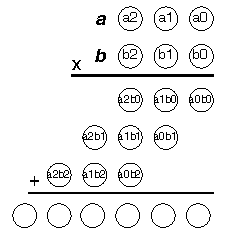
\includegraphics[width=\linewidth]{partialproducts.pdf}
    \caption{Partial products of $a \times b$.}
    \label{fig:partialproducts}
  \end{subfigure}
  \hfill
  \begin{subfigure}{0.44\linewidth}
    \centering
    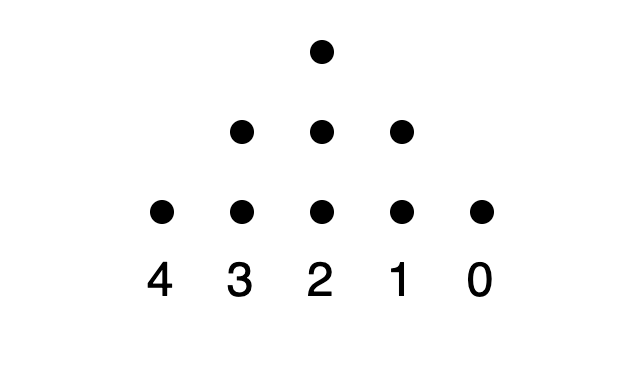
\includegraphics[width=0.95\linewidth]{basic-bh_dots.png}
    \caption{The resulting bit heap.}
    \label{fig:basic-bh}
  \end{subfigure}
  \caption{A $3 \times 3$ unsigned multiplication as a bit heap. Bits are abstract dots and each column can be summed in any order.}
  \label{fig:bitheap-example}
\end{figure}

The bit heap is a data structure that represents the summation of weighted bits \cite{arithmetic_core_generation_bitheaps}. 
Bits are abstract, represented by dots, and are organized into columns based on their weights.
The height of each column corresponds to the number of bit values that need to be summed for that particular weight.
\autoref{fig:bitheap-example} illustrates the bit heap for a $3 \times 3$ unsigned multiplication.

\subsection{Compression Algorithms}
\label{comp_algo}
Compressor trees reduce multiple summands to two using carry-save arithmetic, 
avoiding recursive \acp{cpa} to compute the sum. 
A compressor tree is followed by a single \ac{cpa} that produces the result \cite{application_specific_arithmetic}.
The reduction is carried out by composing compressors, half-adders ($2{:}2$), full-adders ($3{:}2$), or in general any $N{:}M$ compressor with $N \ge M$. 
Different compression algorithms exist, such as the Wallace tree which greedily compresses the bit heap~\cite{wallace_tree} and the Dadda tree, 
that uses the minimal number of compressors to perform the reduction as fast as possible~\cite{dadda_tree}. 
By formalizing the bit heap and the application of compressors to it, we can verify any compression algorithm with a minimal proof. 

\subsection{CIRCT}
\label{sec:circt}
CIRCT is a hardware compiler, based on MLIR, adapting the methods from software compilers to hardware synthesis.
It is capable of expressing different abstraction layers of a hardware design through \textit{dialects}, which
are self-contained sets of operations and types that together form an \ac{ir}.
Separate dialects cover the structure of a design (\texttt{hw}), its
word-level combinational logic (\texttt{comb}), and its gate-level representation (\texttt{synth}), such that a design
can be lowered from RTL-level to gate-level constructs within CIRCT.

CIRCT relies on passes, each of which rewrites the \ac{ir} in place, either optimizing operations within a
dialect or lowering them into a dialect at a lower level of abstraction.
The \texttt{circt-synth} flow chains such passes: it takes a design expressed in \texttt{hw} and \texttt{comb}
and lowers it to an \ac{aig}, which can be passed on to technology mapping.

\section{Formalization}\label{sec:formalization}

To enable verified synthesis, we implement, and prove the correctness of bit heaps.
We begin by defining a symbolic bit representation (\autoref{subsec:bitexpr}) and bit heap (\autoref{subsec:bitheap}) in Lean 4.
We implement basic operations on the bit heap, including evaluating a bit heap to a concrete value, adding and removing bits, and compressing a bit heap. 
These operations then enable us to implement and prove the correctness of the construction of the compressor trees (\autoref{subsec:compression}). 
\sam{Revisit once we've investigated the ordering of sections as didn't reference \autoref{subsec:to_bitheap}?}

\subsection{Symbolic Bit Representations}\label{subsec:bitexpr}
We represent bits of the bit heap via \BitExpr, a language for representing Boolean expressions over symbolic bits.
A \BitExpr can be a Boolean variable, constant, or Boolean operation on \BitExpr values.
\[
\begin{array}{r@{\;}c@{\;}l@{\qquad}l}
\multicolumn{4}{l}{%
  b \in \texttt{Var}  \qquad
  \circledast \in \{\wedge,\vee,\oplus\}}\\[2pt]
\BitExpr \ni c &::=& b \mid 0 \mid 1 \mid \neg c \mid c \circledast c &
\end{array}
\]
To evaluate a \BitExpr, we need to assign values to all the variables in the \BitExpr.
These are supplied by a bit environment $(\sigma : \texttt{Var} \to \mathbb B)$,
which maps each bit variable to its Boolean value. 
The evaluation function $\csem{\cdot} : \BitExpr \to \mathbb B$ evaluates a \BitExpr under a bit environment $\sigma$,
producing a concrete boolean value. It is defined by recursion.
\[
\begin{array}{r@{\;}c@{\;}l}
\csem{b} &=& \sigma(b) \quad \csem{0} = \mathit{false} \quad \csem{1} = \mathit{true}\\
\csem{\neg c} &=& \neg \csem{c} \quad \csem{c_0 \circledast c_1} = \csem{c_0} \circledast \csem{c_1}
\end{array}
\]

\subsection{Bit Heap Data Structure}\label{subsec:bitheap}
A bit heap of width $w$ is a vector of $w$ columns, where the column at index $k$ holds the bits of weight $2^k$. 
A \Col is a set of \BitExpr elements.
\[
\begin{array}{r@{\;}c@{\;}l@{\qquad}l}
\Col \ni \gamma &::=& \{c_0,\dots,c_n\} \\[2pt]
\end{array}
\]

\begin{definition}[Bit heap]
\label{def:bitheap}

Recall that a bit heap is a data structure that is used to represent a summation of weighted bits.
Bits of the same weight are organized into columns, where column $k$ has weight $2^k$.
In implementing the data structure,
we define a \Col as a set of \BitExpr elements,
and a \Heap of width $w$ as a vector of $w$ columns.
\[
  \Heap_w \;\triangleq\; \Vect_w(\Col)
\]
\end{definition}


\paragraph*{Bit Heap Evaluation}
Since a bit heap represents a summation of weighted bits,
we can evaluate the bit heap $h$ under a bit environment $\sigma$ to obtain a concrete value, written as $\csem{h}$.
This is defined by adding up all the bits across all the columns, with bits at column $k$ being evaluated by $\csem{\cdot}$ and weighted by $2^k$. Moreover, since we work with fixed-size bitvectors, all our computations happen modulo $2^w$:
\[
\begin{array}{r@{\;}c@{\;}l}
\csem{\cdot} &:& \Heap_w \to \mathbb{N} \\[2pt]
\csem{h}
  &=& \Bigl(\textstyle\sum_{k<w} 2^{k} \sum_{c \in h_k} \csem{c}\Bigr)
      \bmod 2^{w}
\end{array}
\]

For the purposes of both implementation and proofs by induction,
it is much better to define the evaluation of a bit heap using Horner's method.
Letting $h_k$ denote the $k^{\text{th}}$ column and $v_k = \sum_{c \in h_k} \csem{c}$ denote the value of it:
\begin{equation*}
\begin{split}
  \Bigl( \sum_{k=0}^{w-1} &v_k \cdot 2^{k} \Bigr) \bmod 2^{w}\\
    &= \Bigl( v_0 + 2 \bigl( v_1
      + 2 ( v_2 + \cdots + 2 \, v_{w-1} ) \bigr) \Bigr) \bmod 2^{w}
\end{split}
\end{equation*}
Horner's method cleanly separates the contribution of each column, $v_k$,
and is structurally recursive on the vector of columns, which makes it ameanable to inductive reasoning.

To construct and modify a bit heap we define bit insertion and removal operations.
These are used by higher-level operations such as compression to construct a compressor tree.
Representing each column as a (hash)-set means we cannot add the same bit twice to a column,
however this actually benefits us as we explain below.

\paragraph*{\texttt{addBit}}
Inserting a bit expression $e$ at column $k$ adds $e$ to the set $h_k$.
If $h_k$ already contains bit $e$ we propagate the bit to the next column, since $2^{k}c + 2^{k}c = 2^{k+1}c$.
Effectively, this implies that the bit heap is always in its canonical form,
where the weight of a bit is always equal to the weight of the column it is in.
This canonicalization also optimizes the bit heap during construction automatically,
by re-weighting bits that are added multiple times to the same column, and propagating them to the next column.
If a carry is propagated from the last column, 
it is dropped since we work with fixed-size bit heaps.
This is exactly what we want for reasoning modulo $2^w$.
The correctness of insertion says that adding a bit to the bit heap at weight $k$ 
increases the total value of the bit heap by $2^k$ times the value of the bit expression.

\begin{theorem}[Bit insertion]
\label{thm:addBit} 
For all bit heaps $h : \Heap_w$, bit expressions $e : \BitExpr$, weight $k : \mathbb{N}$,
and environment $\sigma : \mathcal{V} \to \mathbb{B}$,
$\hsem{\mathtt{addBit}(k, e, h)}
 =
\bigl(\hsem{h}
      + 2^{k}\cdot \csem{e} \bigr) \bmod 2^{w}.
$
\end{theorem}
The proof follows by functional induction on \texttt{addBit}, following the carry propagation described above.

\paragraph*{\texttt{removeBit}}
Removing a bit expression $e$ at column $k$ removes $e$ from the set $h_k$.
Removal is only meaningful if $e\in h_k$; therefore, we require that the bit to be removed is present in the column.
This is encoded as an explicit hypothesis of the correctness theorem for bit removal (\autoref{thm:removeBit}).
Under this hypothesis, removing a bit $e$ from column $k$ decreases the value of the bit heap by $2^k \csem{e}$.
\begin{theorem}[Bit removal]
\label{thm:removeBit}
For all $h : \Heap_w$, $k : \mathbb{N}$, $c : \BitExpr$ and
$\sigma : \mathcal{V} \to \mathbb{B}$ with $c \in h_k$,
\[
  \hsem{\mathtt{removeBit}(k, c, h)}
  \;=\;
  \bigl(\hsem{h}
        - 2^{k}\cdot\lift{\csem{c}}\bigr) \bmod 2^{w}.
\]
\end{theorem}
The proof is a simple algebraic argument and does not require induction, since the removal only affects a single column.

\begin{table*}
  \centering
  \caption{Compression steps on an input heap $h$, producing $h'$.
           $\maj$ denotes the majority function
           $(i \wedge j) \vee (i \wedge l) \vee (j \wedge l)$.}
  \label{tab:steps}
  \begin{tabular}{@{}lll@{}}
  \toprule
  Step & Applicability & Effect \\
  \midrule
  $\HA(k,i,j)$
    & $i,j \in h_k$, $i \neq j$, $k<w$
    & $\begin{aligned}
        g_1 &= \mathtt{removeBit}(k,j,\mathtt{removeBit}(k,i,h)) \\
        g_2 &= \mathtt{addBit}(k,i\oplus j,g_1) \\
        h'  &= \mathtt{addBit}(k+1,i\wedge j,g_2)
      \end{aligned}$ \\[6pt]
\midrule
  $\FA(k,i,j,l)$
    & $i,j,l \in h_k$, pairwise distinct, $k<w$
    & $\begin{aligned}
        g_1 &= \mathtt{removeBit}(k,j,\mathtt{removeBit}(k,i,h)) \\
        g_2 &= \mathtt{removeBit}(k,l,g_1) \\
        g_3 &= \mathtt{addBit}(k,i\oplus j\oplus l,g_2) \\
        h'  &= \mathtt{addBit}(k+1,\maj(i,j,l),g_3)
      \end{aligned}$ \\
  \bottomrule
  \end{tabular}
\end{table*}


\subsection{From Word-Level Arithmetic to Bit Heaps}\label{subsec:to_bitheap}
So far, we have defined the bit heap data structure and its operations, and proved that they preserve the semantics of bit heap evaluation.
To use the bit heap to synthesize efficient and provably correct circuits for word-level arithmetic, we require a verified translation from arithmetic to a bit heap.
We represent such arithmetic expressions as \Arith, a minimal symbolic
representation of word-level arithmetic. 
We will define a function $\mathsf{toBitHeap}$ that converts an \Arith expression into a bit heap.
This conversion then lets us to apply compressor trees to synthesize efficient circuits (\autoref{subsec:compression}).
First, we define the syntax and semantics of \Arith.
Then, we prove that the semantics of the resulting bit heap are equal to the semantics of the original \Arith.

\Arith is a word-level representation supporting variables,
variadic addition and two-input multiplication.
This allows us to represent nested arithmetic expressions, like $a\times b + c$.
We also support zero/sign-extension of variables, as this lets our multiplication preserve the full precision of the result.
\begin{align*}
&b \in \texttt{Var}_{\texttt{Arith}} \qquad v, w \in \mathbb{N}^{+}\\
&\mathtt{ArithCircuit}_w \ni a ::= \\
&\quad \mid b \mid \mathsf{zext}(i, b) \mid \mathsf{sext}(i, b) \mid \mathsf{add}[a_0,\dots,a_{n-1}] \mid \mathsf{mul}[a_0, a_1]
\end{align*}

The \Arith variables are assigned a value by a variable environment $\rho : \texttt{Var}_{\texttt{Arith}} \to \mathtt{BitVec}\ w$, mapping each variable to Lean's built-in bitvector type of width $w$.
\sam{We should make it clear that everything gets assigned to $w$-bits?}
A variable evaluates to the word the environment assigns it.
A zero-extended variable $\mathsf{zext}(b,w')$, where $w'\leq w$, evaluates by truncating that word to its lowest $w'$-bits and zero-extending the result back to the width of the \Arith expression.
A sign-extended variable $\mathsf{sext}(b,w')$, where $w' \leq w$, truncates in the same way, but extends the result back to width $w$ by replicating the sign bit, i.e. bit $b-1$ of the word.
The addition and multiplication operations in \Arith are interpreted following standard bitvector arithmetic.

We construct a bit heap by structural recursion on the arithmetic expression. 
Each recursive call returns a width-$w$ bit heap representing its subexpression modulo $2^w$.
Variables and zero-/sign-extended variables produce a single row bit heap.
Addition merges the recursively constructed operand bit heaps, increasing the bit heaps height or automatically propagating duplicated addends, i.e., $x+x = 2x$.
The multiplication of two bit heaps, $h$ and $g$, produces a single bit heap containing for every $e \in h_i$ and $f \in g_j$ a bit $e \land f$ in column $i+j$. Any bits for which $i+j\geq w$ are discarded.
We formally prove that the translation from \Arith expressions to bit heaps preserves their fixed-width arithmetic semantics.

\begin{theorem}[Construction]\label{thm:tobitheap}
For all $a : \mathtt{ArithCircuit}_w$ and all $\rho : \texttt{Var}_{\texttt{Arith}}\to
\mathtt{BitVec}\ w$, let $\sigma$ denote the bit environment induced
by $\rho$, then
\[
  \hsem{\mathsf{toBitHeap}(a)} \;=\; \bvsem{a}.
\]
\end{theorem}

The proof uses structural indusction handling each \Arith operation separately. 
The proofs for variables and their zero-extension are trivial. 
The sign-extended case requires an induction argument on the number of replicated columns,
for which we give a closed form for the value of the heap after $k$ sign columns have been added:
it is $x_{[0,b)}$ when the sign bit is clear, and $x_{[0,b)} + (2^{b+k} - 2^{b})$ when it is set.
Each further column contributes exactly one more copy of the sign bit at weight $2^{b+k}$, which proves the induction step,
and the closed form stays below $2^{w}$ as long as $b + k \leq w$, so the truncation in the bit heap semantics never wraps around.
Instantiating the closed form at $k = w - b$ yields precisely the value of the sign-extended word.
\sam{This proof for sign-extension case became very confusing...}
The addition proof is simpler and uses the identity $\sum_i h_i 2^i + \sum_j  g_j 2^j = \sum_k (h_i + g_i) 2^k$.
Similarly, partial products are proven equal using the identity $\sum_i x_i 2^i \cdot \sum_j y_j 2^j = \sum_{i,j} x_i y_j 2^{i+j}$.

Overall, we verified the conversion from word-level arithmetic to a bit heap (\autoref{thm:tobitheap}).
Other than the multiplier, which created AND gates to compute the partial product bits, 
we have not constructed any logic gates.
What remains is to construct and verify the compressor tree for a given bit heap.


\subsection{Compression Algorithms For Fast Arithmetic}\label{subsec:compression}

To compress the bit heap we apply a tree of compressors (half and full adders),
which reduce its height to two.
The compressor tree is followed by a single \ac{cpa} that sums the remaining two rows.
We proceed by first proving that applying a single compressor to a bit heap preserves its evaluated value,
then prove correct the composition of compressors.
These foundational proofs make it easy to prove Wallace's~\cite{wallace_tree} and Dadda's~\cite{dadda_tree} compression algorithms.

Concretely, any compression algorithm produces a sequence of compression steps.
Formally, we define a \Step as either a half adder or a full adder. Each compressor takes
the column index, $k$, and the bits ($c_1, c_2, c_3$) it consumes as arguments.
\[
\begin{array}{r@{\;}c@{\;}l@{\qquad}l}
\Step \ni s &::=& \HA(k,c_1,c_2) \mid \FA(k,c_1,c_2,c_3) &
\end{array}
\]
Each compressor is accompanied by an applicability condition and maps to a sequence 
of \texttt{addBit}/\texttt{removeBit} operations (\autoref{tab:steps}).
Writing $h \xrightarrow{s} h'$ for the heap $h'$ obtained by applying step $s$ to $h$, we prove that any applicable step preserves the value of the bit heap.
\begin{theorem}[Half/Full Adder Correct]
\label{thm:step-correct}
For all $h : \Heap_w$, and $s : \Step$ if $s$ obeys the applicability conditions (\autoref{tab:steps}) and $h \xrightarrow{s} h'$, then $\hsem{h} \;=\; \hsem{h'}$.
\end{theorem}

Proceeding one compressor type at a time, this proof rewrites the goal using the lemmas for 
\texttt{addBit}/\texttt{removeBit} (\autoref{thm:addBit}, \autoref{thm:removeBit}) reducing the
goal to an arithmetic identity over the Boolean values of bits.
This is then discharged by case analysis on the Booleans, and some arithmetic reasoning. \sam{Why can we not just discharge this with bv decide?}

As an example, consider the step $\HA(k,i,j)$, which removes $i$ and $j$ from column $k$,
and adds $i \oplus j$ at column $k$ and $i \wedge j$ at column $k{+}1$ (\autoref{tab:steps}).
Writing $h'$ for the resulting heap, the theorem states that the value of the heap is preserved:
\[
  \hsem{h'} \;=\; \hsem{h}.
\]
Unfolding $h'$ by rewriting first \texttt{addBit} (\autoref{thm:addBit}) and \texttt{removeBit} (\autoref{thm:removeBit}),
then removing intermediate $\bmod$ operations we obtain an arithmetic identity:
\begin{equation*}
\begin{split}
  \bigl(\hsem{h}
    &- 2^{k}\csem{i}
     - 2^{k}\csem{j}\\
    &+ 2^{k}\csem{i \oplus j}
     + 2^{k+1}\csem{i \wedge j}\bigr) \bmod 2^{w}\\
  &\;=\; \hsem{h} \bmod 2^{w}.
\end{split}
\end{equation*}
The proof follows by case analysis on the four possible values of $i$ and $j$.
The full adder case follows the same structure.

Having established that each individual step preserves the value of the heap, we now consider
sequences of steps.
Formally, a chain of compressors is an ordered list of compression steps, where each step is a half or full adder,
and is either empty or a step followed by a chain:
\[
\begin{array}{r@{\;}c@{\;}l@{\qquad}l}
\Chain \ni S &::=& [\,] \mid s :: S &
\end{array}
\]

We will notate this as $S \equiv s_0 :: s_1 \dots :: s_{n-1}$ for a chain of $n$ steps.
We write $h \xrightarrow{S} h'$ for the application of a chain $S$ to a bit heap $h$, producing a new bit heap $h'$.
This can be broken down into a sequence of applications $h = h_0 \xrightarrow{s_0} h_1 \xrightarrow{s_1} \dots \xrightarrow{s_{n-1}}  h'$.
We call a chain \emph{well formed}, iff, at each step $h_i \xrightarrow{s_i} h_{i+1}$, the applicability conditions of the step $s_{i}$
are satisfied by the intermediate bit heap $h_i$.
As above, the applicability conditions (\autoref{tab:steps}) ensure that the bits consumed by the step $s_i$ are present in the bit heap $h_i$,
and that the consumed bits are pairwise distinct.
This well-formedness condition allows us to prove the key chain correctness theorem (\autoref{thm:chain-correct}),
which states that any well-formed chain preserves the value of the bit heap.

\begin{figure*}[t]
  \centering
  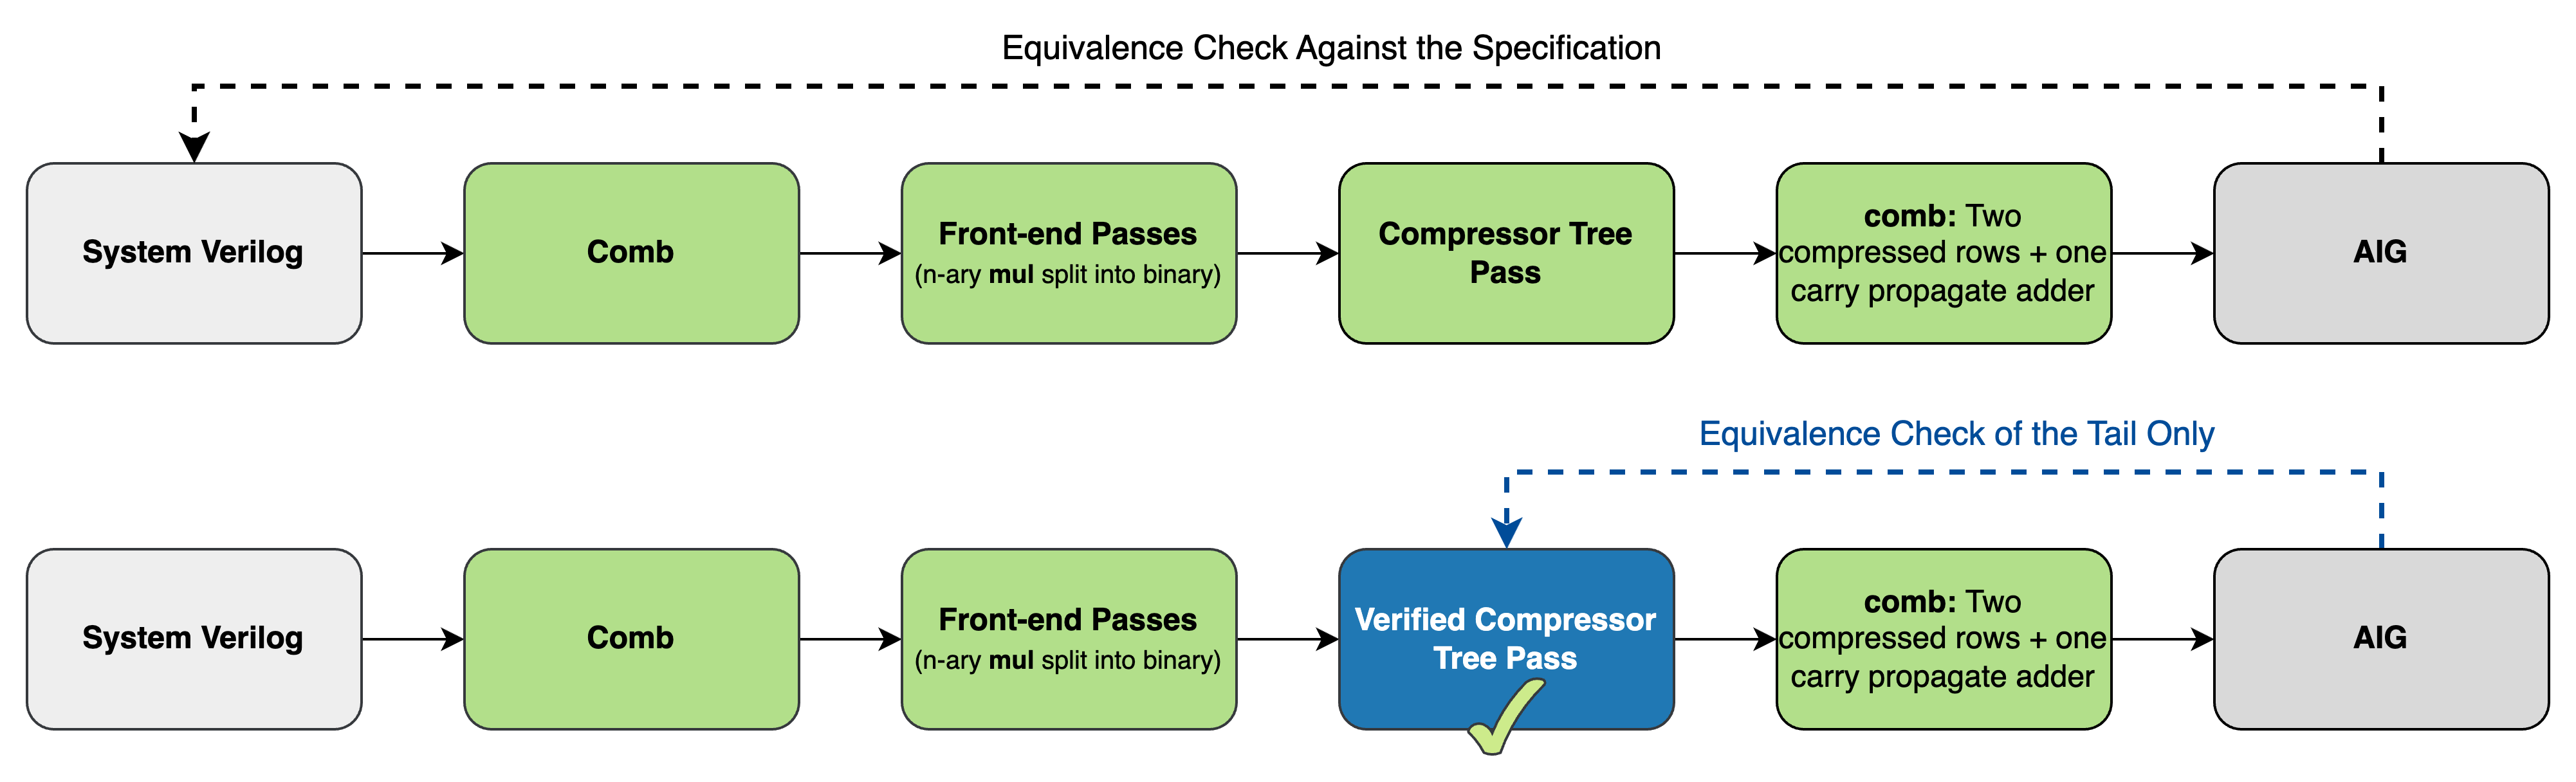
\includegraphics[width=0.72\textwidth]{flow-diagram.png}
  \caption{The baseline \texttt{circt-synth} flow (top) and ours (bottom). Both share
  CIRCT's front-end passes and its \texttt{comb}-to-\ac{aig} lowering; we replace only the
  compressor-tree pass, whose result is guaranteed by \autoref{thm:tobitheap-compression},
  and check the remaining tail against the baseline netlist with a SAT solver.}
  \label{fig:flow-comparison}
\end{figure*}

\begin{theorem}[Chain Correctness]
\label{thm:chain-correct}
For all $h : \Heap_w$ and $S: \Chain$ is well-formed for $h$,
\[
  \forall \sigma,\quad
  \hsem{S(h)} \;=\; \hsem{h} .
\]
\end{theorem}

Chain correctness (\autoref{thm:chain-correct}) is proven by induction on the length of the chain.
The base case, when the chain has length $0$, is trivial, since the heap is unchanged.
For the induction step, the new step $s_{i+1}$'s correctness is justified by the step correctness theorem
proven above (\autoref{thm:step-correct}),
and the induction hypothesis is used to prove that the other steps preserve the value of the heap.

This shows that \emph{any} well-formed chain preserves the value of the bit heap.
It should we noted that we do not verify compression algorithms themselves.
But instead we verify that the chain of compressors generated by a compressor algorithm preserves the value at the run-time.
So we define $\mathsf{applyChainSafe}$, which applies a chain step by step, checks the conditions of each step against the bit heap it
has reached, and returns $\mathsf{none}$ if a step does not apply.
We then prove that a successful run preserves the value:
\[
  \mathsf{applyChainSafe}(S, h) = \mathsf{some}\ h'
  \quad\Longrightarrow\quad
  \forall \sigma,\; \hsem{h'} = \hsem{h}.
\]

Dadda's algorithm is a plain Lean function with no correctness theorem of its own.
It proposes a chain, and the check decides whether that chain is used.
Any other compression algorithm can take its place without further proof, since only the chain it produces is checked.
This is the check the CIRCT pass of \autoref{sec:integration} runs.

\begin{theorem}[Bit Heap Compression]
\label{thm:tobitheap-compression}
For all $a : \mathtt{ArithCircuit}_w$, all $\rho : \mathbb{N} \to
\mathtt{BitVec}\ w$, and $S: \Chain$ is well-formed for $h$,
\[
  \forall \sigma,\quad
  \hsem{S(\mathsf{toBitHeap}(a))} \;=\; \bvsem{a}.
\]
\end{theorem}

Finally, we prove that compression of word-level arithmetic expressions preserves the value (\autoref{thm:tobitheap-compression}).
The proof is a corollary of \autoref{thm:tobitheap} and \autoref{thm:chain-correct}.

This now completes the overall proof of correctness of compression algorithms.
We will use this to synthesize fast and verified multiplier circuits in CIRCT framework.
The next sections will explain the integration into CIRCT and the results of the verified synthesis of multipliers.

\section{Integration}
\label{sec:integration}

We integrate our verified synthesizer into the CIRCT compiler framework, and make our contributions open-source.
CIRCT's \texttt{circt-synth} flow lowers the word-level \texttt{comb} dialect to an
\ac{aig}; within that flow, a datapath engine rewrites arithmetic operations into
compressor trees in a dedicated pass.
We replace exactly this pass and leave the rest of the flow untouched, so that our
pipeline is a drop-in alternative to CIRCT's and the two are directly comparable.
\autoref{fig:flow-comparison} shows the two flows side by side, and marks which stages
are verified in Lean and which are discharged by the SAT check on the tail.

Using circt-verilog, we write the SystemVerilog design into CIRCT's RTL dialects, namely the comb.
Then, a pass matches arbitrary sums of products, that is, expressions built from two-operand
\texttt{comb.mul} and $n$-operand \texttt{comb.add} for $n \geq 3$ (e.g. $a*b+c*d+e$),
but it does not match for two-operand additions, since they are already carry-propagate adders and are left alone, whereas
variadic multiplications are decomposed into binary ones by an existing CIRCT pass beforehand.

For each matched \ac{sop} expression, our tool builds the corresponding bit heap and compresses
it with the Dadda algorithm.
The resulting chain is replayed through the well-formedness checker. 
A successful check discharges the proof obligations required to apply \autoref{thm:tobitheap-compression}, which guarantees
that the compressed bit heap denotes the same value as the original expression.
The pass then emits the compressor tree as gates, leaving two compressed rows and a single
carry-propagate adder that CIRCT's existing synthesizer implements.
This adder, together with the local optimizations such as \ac{cse} that CIRCT applies afterwards,
is the only part of the circuit our proof does not cover.
We discharge this tail with a SAT solver, checking the netlist CIRCT produces
against the circuit generated by our verified core.
Because the two circuits differ only in the tail, the check is far cheaper than
equivalence checking a multiplier against its specification, since the checker
does not need to relate the gate-level constructs to their word-level expressions, which is the hardest part for the existing methods.
Outside the circuit itself, the front-end from Verilog, as well as the hand-off to Lean and
the return, remain unverified.
This leaves a small trusted base, as these parts are syntax translations between
SystemVerilog, \texttt{comb} operations and \texttt{ArithCircuit} constructors.
\autoref{fig:flow-comparison} depicts this flow for both the unverified and verified paths.

\section{Evaluation}\label{sec:evaluation}
We evaluate our results on two metrics, the circuit quality and the time needed to verify the circuits.
We compare our results against the CIRCT datapath pass that we replace.
\sam{We should provide some evidence that we really isolate the hard part with our Lean synthesizer. 
Namely, a reviewer might ask well what happens if you decompose the original CIRCT problem into two separate SMT problems using an identical cutpoint as you've used.
We can handle this query by showing that even for a simple multiplier this step does not converge with an SMT solver.}

We use a benchmark consisting of 22 datapath designs\footnote{\url{https://github.com/cowardsa/DatapathBench}},
spanning multi-operand addition and multiplication, dot-products and fused multiply-add variants in signed and unsigned forms.
We instantiate each design at 8, 16, 32-bit operand widths.

We synthesize the designs using both the unverified CIRCT path and our verified datapath generator.
Both are technology mapped to the ASAP 7nm library \cite{asap7} using Mockturtle, and we report the total cell area and critical-path delay.
For the verification of the unverified path and the tail of our verified circuit, we use Bitwuzla SMT solver \cite{bitwuzla}

\autoref{tab:qor-and-time-16} reports area and delay at 16 bits, normalized to the results of the unverified CIRCT path.
The netlists our pass produces are close to CIRCT's. The geometric mean is $\geoAreaSixteen\times$ in area and $\geoDelaySixteen\times$ in delay at 16 bits,
with the gap being stable for other bit widths as well ($\geoAreaThirtyTwo\times$ / $\geoDelayThirtyTwo\times$ at 32 bits, $\geoAreaEight\times$ / $\geoDelayEight\times$ at 8 bits).

The existing gap in circuit quality is not an inherent limitation of our workflow.
CIRCT's datapath engine applies certain optimizations we have not yet implemented, notably Booth encoding and sign-extension optimizations \cite{application_specific_arithmetic}. \sam{cite?}
This is also revealed on our performance on signed benchmarks.

\autoref{tab:qor-and-time-16} reports how both of flows perform on total verification time. 
For the unverified path, we verify the resulting \ac{aig} against the word-level Verilog design,
and for the verified path, we verify the front-end passes, the tail of the circuit -final-stage adder and simple optimizations, against the intermediate circuit generated by our Lean framework.

The results show that we are able to verify circuits that the standard flow cannot verify\osman{funny thing, we are not faster on the ones that the standard flow can already verify, because it already cannot verify most},
with out flow verifying 11 more circuits than the standard flow, we show the effectiveness of our approach on verification.

\begin{table}
  \centering
  \caption{Synthesis quality and proof cost at 16-bit operand width. \textsc{Verified\,/\,Datapath} is post-technology-mapping ASAP7 area and delay relative to CIRCT's Datapath dialect, so below $1.00$ favours the verified lowering. \textsc{Time to trust} is synthesis plus equivalence checking, in seconds: \textsc{Standard} proves the result against the original Verilog, re-checking the whole pipeline, while \textsc{Verified} proves it against the Lean snapshot, leaving only the unverified comb-to-AIG tail. $\times$ marks a solver timeout. $^{\dagger}$ marks signed benchmarks.}
  \label{tab:qor-and-time-16}
  \small
  \setlength{\tabcolsep}{4pt}
  \begin{tabular}{lrrrr}
    \toprule
    & \multicolumn{2}{c}{Verified\,/\,Datapath} & \multicolumn{2}{c}{Time to trust (s)} \\
    \cmidrule(lr){2-3} \cmidrule(lr){4-5}
    Benchmark & Area & Delay & \textsc{Standard} & \textsc{Verified} \\
    \midrule
    AddMop & 1.00 & 1.06 & 0.45 & 0.35 \\
    AddMulSgn$^{\dagger}$ & 1.19 & 1.54 & $\times$ & $\times$ \\
    AddMulUns & 1.02 & 1.21 & $\times$ & $\times$ \\
    AddThree & 1.00 & 0.94 & 0.24 & 0.34 \\
    AddThreeSgn$^{\dagger}$ & 1.00 & 0.94 & 0.20 & 0.34 \\
    AlphaBlend & 0.97 & 1.13 & $\times$ & $\times$ \\
    CarrySaveCompare & 1.02 & 0.98 & $\times$ & 5.35 \\
    CarrySaveSelect & 1.06 & 1.09 & $\times$ & 2.74 \\
    DotProduct & 1.01 & 1.02 & $\times$ & 54.12 \\
    DotProductSgn$^{\dagger}$ & 1.64 & 1.04 & $\times$ & $\times$ \\
    Fma & 1.01 & 1.05 & $\times$ & 3.90 \\
    FmaSgn$^{\dagger}$ & 1.61 & 1.14 & $\times$ & $\times$ \\
    FmaShare & 1.01 & 1.17 & $\times$ & 35.82 \\
    FmaShareSgn$^{\dagger}$ & 1.48 & 1.38 & $\times$ & $\times$ \\
    Fmaa & 1.00 & 0.95 & $\times$ & 2.31 \\
    FmaaSgn$^{\dagger}$ & 2.03 & 1.28 & $\times$ & 38.64 \\
    MulAddSgn$^{\dagger}$ & 1.57 & 1.14 & $\times$ & 13.21 \\
    MulAddUns & 1.01 & 1.07 & $\times$ & 1.68 \\
    MulThree & 1.01 & 1.14 & $\times$ & 21.82 \\
    MulThreeSgn$^{\dagger}$ & 1.01 & 1.14 & $\times$ & 22.01 \\
    SqrSgn$^{\dagger}$ & 1.79 & 1.18 & 13.93 & 23.60 \\
    SqrUns & 1.48 & 1.13 & 9.18 & 18.62 \\
    \bottomrule
  \end{tabular}
\end{table}

% \begin{table}
%   \centering
%   \caption{Per-benchmark area and delay at 32-bit operand width after technology
%   mapping to ASAP7, reported by Mockturtle's mapper. Both columns are normalised to the
%   unverified CIRCT datapath pass, so $1.00$ is parity and values below $1.00$
%   favour our flow. Geometric means are taken over all 22 benchmarks.
%   $^{\dagger}$ marks signed benchmarks.}
%   \label{tab:verified-full-32-asap7}
%   \small
%   \begin{tabular}{lrr}
%     \toprule
%     Benchmark & Area & Delay \\
%     \midrule
%     AddMop & 1.00 & 1.08 \\
%     AddMulSgn$^{\dagger}$ & 1.17 & 1.35 \\
%     AddMulUns & 1.04 & 1.21 \\
%     AddThree & 1.03 & 1.06 \\
%     AddThreeSgn$^{\dagger}$ & 1.03 & 1.07 \\
%     AlphaBlend & 0.99 & 1.11 \\
%     CarrySaveCompare & 0.98 & 1.02 \\
%     CarrySaveSelect & 1.20 & 1.13 \\
%     DotProduct & 0.99 & 0.96 \\
%     DotProductSgn$^{\dagger}$ & 1.66 & 1.25 \\
%     Fma & 0.96 & 1.00 \\
%     FmaSgn$^{\dagger}$ & 1.61 & 1.13 \\
%     FmaShare & 1.04 & 1.22 \\
%     FmaShareSgn$^{\dagger}$ & 1.58 & 1.30 \\
%     Fmaa & 0.86 & 1.02 \\
%     FmaaSgn$^{\dagger}$ & 1.54 & 1.38 \\
%     MulAddSgn$^{\dagger}$ & 1.59 & 1.15 \\
%     MulAddUns & 0.98 & 1.02 \\
%     MulThree & 1.06 & 1.19 \\
%     MulThreeSgn$^{\dagger}$ & 1.06 & 1.19 \\
%     SqrSgn$^{\dagger}$ & 1.52 & 1.07 \\
%     SqrUns & 1.55 & 1.24 \\
%     \midrule
%     Geometric mean (32-bit) & 1.17 & 1.14 \\
%     Geometric mean (16-bit) & 1.21 & 1.12 \\
%     Geometric mean (8-bit) & 1.21 & 1.10 \\
%     \bottomrule
%   \end{tabular}
% \end{table}

% \begin{table}
%   \centering
%   \caption{Total time to obtain a trusted netlist at 8-bit operand width, in seconds: synthesis plus equivalence checking. \textsc{Standard} proves the synthesised AIG against the original Verilog, so the whole pipeline is re-checked; \textsc{Verified} proves it against the Lean snapshot, leaving only the unverified comb-to-AIG tail. $\times$ marks a solver timeout. $^{\dagger}$ marks signed benchmarks.}
%   \label{tab:verify-time-8}
%   \small
%   \begin{tabular}{lrr}
%     \toprule
%     Benchmark & \textsc{Standard} & \textsc{Verified} \\
%     \midrule
%     AddMop & 0.66 & 0.22 \\
%     AddMulSgn$^{\dagger}$ & $\times$ & 18.12 \\
%     AddMulUns & $\times$ & 9.46 \\
%     AddThree & 0.64 & 0.23 \\
%     AddThreeSgn$^{\dagger}$ & 0.14 & 0.20 \\
%     AlphaBlend & $\times$ & 123.98 \\
%     CarrySaveCompare & 0.51 & 0.32 \\
%     CarrySaveSelect & 2.31 & 0.60 \\
%     DotProduct & $\times$ & 1.53 \\
%     DotProductSgn$^{\dagger}$ & $\times$ & $\times$ \\
%     Fma & 70.48 & 0.65 \\
%     FmaSgn$^{\dagger}$ & 55.81 & 5.91 \\
%     FmaShare & 13.43 & 1.16 \\
%     FmaShareSgn$^{\dagger}$ & 15.75 & 4.85 \\
%     Fmaa & $\times$ & 0.46 \\
%     FmaaSgn$^{\dagger}$ & $\times$ & 22.43 \\
%     MulAddSgn$^{\dagger}$ & 248.05 & 3.80 \\
%     MulAddUns & 174.39 & 0.45 \\
%     MulThree & 10.05 & 2.03 \\
%     MulThreeSgn$^{\dagger}$ & 9.98 & 2.10 \\
%     SqrSgn$^{\dagger}$ & 0.18 & 0.34 \\
%     SqrUns & 0.16 & 0.27 \\
%     \bottomrule
%   \end{tabular}
% \end{table}
% \begin{table}
%   \centering
%   \caption{Total time to obtain a trusted netlist at 16-bit operand width, in seconds: synthesis plus equivalence checking. \textsc{Standard} proves the synthesised AIG against the original Verilog, so the whole pipeline is re-checked; \textsc{Verified} proves it against the Lean snapshot, leaving only the unverified comb-to-AIG tail. $\times$ marks a solver timeout. $^{\dagger}$ marks signed benchmarks.}
%   \label{tab:verify-time-16}
%   \small
%   \begin{tabular}{lrr}
%     \toprule
%     Benchmark & \textsc{Standard} & \textsc{Verified} \\
%     \midrule
%     AddMop & 0.44 & 0.24 \\
%     AddMulSgn$^{\dagger}$ & $\times$ & $\times$ \\
%     AddMulUns & $\times$ & $\times$ \\
%     AddThree & 0.21 & 0.22 \\
%     AddThreeSgn$^{\dagger}$ & 0.17 & 0.22 \\
%     AlphaBlend & $\times$ & $\times$ \\
%     CarrySaveCompare & $\times$ & 5.57 \\
%     CarrySaveSelect & $\times$ & 2.77 \\
%     DotProduct & $\times$ & 58.02 \\
%     DotProductSgn$^{\dagger}$ & $\times$ & $\times$ \\
%     Fma & $\times$ & 3.66 \\
%     FmaSgn$^{\dagger}$ & $\times$ & $\times$ \\
%     FmaShare & $\times$ & 36.59 \\
%     FmaShareSgn$^{\dagger}$ & $\times$ & $\times$ \\
%     Fmaa & $\times$ & 2.20 \\
%     FmaaSgn$^{\dagger}$ & $\times$ & 175.88 \\
%     MulAddSgn$^{\dagger}$ & $\times$ & 20.57 \\
%     MulAddUns & $\times$ & 1.59 \\
%     MulThree & $\times$ & 22.86 \\
%     MulThreeSgn$^{\dagger}$ & $\times$ & 22.72 \\
%     SqrSgn$^{\dagger}$ & 14.65 & 26.24 \\
%     SqrUns & 11.78 & 19.95 \\
%     \bottomrule
%   \end{tabular}
% \end{table}

% \begin{table}
%   \centering
%   \caption{Total time to obtain a trusted netlist at 32-bit operand width, in seconds: synthesis plus equivalence checking. \textsc{Standard} proves the synthesised AIG against the original Verilog, so the whole pipeline is re-checked; \textsc{Verified} proves it against the Lean snapshot, leaving only the unverified comb-to-AIG tail. $\times$ marks a solver timeout. $^{\dagger}$ marks signed benchmarks.}
%   \label{tab:verify-time-32}
%   \small
%   \begin{tabular}{lrr}
%     \toprule
%     Benchmark & \textsc{Standard} & \textsc{Verified} \\
%     \midrule
%     AddMop & 1.15 & 0.35 \\
%     AddMulSgn$^{\dagger}$ & $\times$ & $\times$ \\
%     AddMulUns & $\times$ & $\times$ \\
%     AddThree & 0.35 & 0.29 \\
%     AddThreeSgn$^{\dagger}$ & 0.35 & 0.31 \\
%     AlphaBlend & $\times$ & $\times$ \\
%     CarrySaveCompare & $\times$ & 169.87 \\
%     CarrySaveSelect & $\times$ & 29.72 \\
%     DotProduct & $\times$ & $\times$ \\
%     DotProductSgn$^{\dagger}$ & $\times$ & $\times$ \\
%     Fma & $\times$ & 54.21 \\
%     FmaSgn$^{\dagger}$ & $\times$ & $\times$ \\
%     FmaShare & $\times$ & $\times$ \\
%     FmaShareSgn$^{\dagger}$ & $\times$ & $\times$ \\
%     Fmaa & $\times$ & 22.87 \\
%     FmaaSgn$^{\dagger}$ & $\times$ & $\times$ \\
%     MulAddSgn$^{\dagger}$ & $\times$ & $\times$ \\
%     MulAddUns & $\times$ & 21.48 \\
%     MulThree & $\times$ & $\times$ \\
%     MulThreeSgn$^{\dagger}$ & $\times$ & $\times$ \\
%     SqrSgn$^{\dagger}$ & $\times$ & $\times$ \\
%     SqrUns & $\times$ & $\times$ \\
%     \bottomrule
%   \end{tabular}
% \end{table}

\section{Related Work}
\citet{arithmetic_core_generation_bitheaps} propose the bit heap as the central data structure
of arithmetic designs, giving an exposition of bit heaps and how they can be used in multiplier synthesis on FPGAs.
FloPoCo~\cite{application_specific_arithmetic}, an open-source datapath generator written in C++ that produces
arithmetic circuits in VHDL, is built on the framework that \cite{arithmetic_core_generation_bitheaps} lay out,
and thus on the same bit heap abstraction and compression techniques that we formalize in this paper.
However, neither provides formal correctness guarantees, and the generated circuits have to be validated by testing.

\citet{sca} presents a method based \ac{sca} approach to verify multiplication circuits, 
using backwards rewriting of polynomials at the gate level, employing a dynamic strategy consisting of sub-circuit detection and phase signal adjusting.
\citet{trace} extend this line beyond multipliers with TRACE, an \ac{sca} engine that combines
different substitution orders with polynomial compression techniques, namely phase optimization
and conflict analysis, and verifies adders and multiply-accumulate units as well.

In their work, \citet{mertcan_acl2multipliers} prove correctness of integer multiplication circuits using a rewrite-based method in ACL2. 
Their approach can verify different partial-product generation and compression tree algorithms scaling to $1024\times1024$ bit multipliers in minutes. 
Similar to our approach, their implementation of the tool in a theorem prover guarantees the correctness of the verification tool.

A line of research focuses on proving \ac{hls} tools correct. 
Graphiti \citet{graphiti} is a graph-rewriting framework in Lean 4 to formally reason about optimizations on dataflow circuits.
Integrated into an existing HLS tool, Graphiti provides a verified rewriting engine that ensures the composition of verified rewrites refines the original behaviour.



\section{Conclusion and Future Work}
This paper presents a verified datapath synthesis engine integrated into CIRCT.
By formalizing datapath synthesis steps with using bit heaps as the core data structure in Lean 4,
we provide machine-checked correctness guarantees on the arithmetic circuits we generate.
Our insight is that the most challenging verification task in datapath synthesis is the verification of the multipliers due to complex compressor trees.
We therefore formally verify this stage of datapath synthesis, and leave the remaining proof obligations to an SMT-solver, which discharges them easily.
At 16-bits, our approach can verify 16 of 22 designs within the timeout 
while only being 1.21 times larger and 1.12 times slower than unverified method,
whereas the SMT-based baseline can only verify 5 of the designs.
We make all our contributions open-source on (this link).\osman{should we put a link here? if so how to appropriately anonymize it?}

Future work will address the missing optimizations on bit heaps and datapath synthesis.
Namely Booth encoding, sign-extension related optimizations opportunities, and extend our formalization
with timing-aware compression, in which the arrival of each bit is accounted for during the compression.


%% Acknowledgments. IEEEtran has no \begin{acks} or \grantsponsor/\grantnum;
%% IEEE uses an unnumbered section. Suppressed for anonymous review.
\ifx\acmversion\acmversionanonymous
\else
\section*{Acknowledgments}
  This material is based upon work supported by the National Science
  Foundation under Grant No.~nnnnnnn and Grant No.~mmmmmmm.  Any opinions,
  findings, and conclusions or recommendations expressed in this material are
  those of the author and do not necessarily reflect the views of the
  National Science Foundation.
\fi

%% Bibliography
\bibliography{references}

\end{document}
